\paragraph{Giả thiết}
    Cho hệ thống như hình \ref{Fig:baitap4-2binhchua}: Các lưu lượng ra $q_1$ và $q_0$ được xác định như sau: $q_1 = \dfrac{h_1 - h_2}{R_1}$ và $q_0 = \dfrac{h_2}{R_2}$
    \begin{figure}[htp]
        \begin{center}
            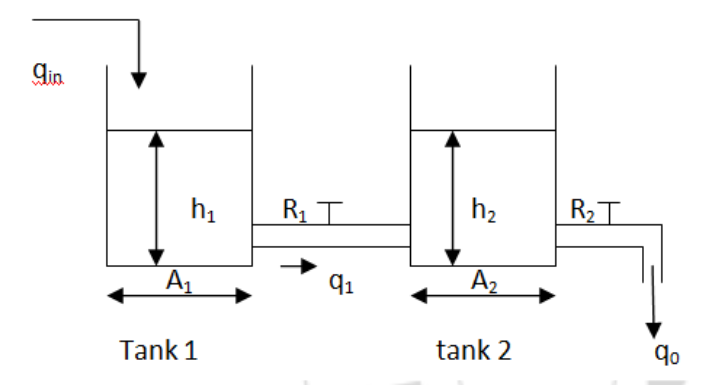
\includegraphics[scale=.5]{baitap4-2binhchua}
        \end{center}
        \caption{Hệ thống 2 bình chứa} \label{Fig:baitap4-2binhchua}
    \end{figure}

\paragraph{Yêu cầu}
    \begin{enumerate}[a.]
        \item Xác định các biến vào, biến ra, biến điều khiển, biến cần điều khiển và biến nhiễu.
        \item Viết phương trình động học cho mức chất lỏng trong bồn chứa.
        \item Nếu phương trình phi tuyến hãy tuyến tính hóa phương trình xây dựng được xung quanh vị trí cân bằng dựa trên phương pháp khai triển Taylor.
        \item Xác định hàm truyền $G(s) = \dfrac{H_2(s)}{Q_{in}(s)}$
    \end{enumerate}

\paragraph{Bài giải}
    \begin{enumerate}[\it a.]
        \item \textit{Xác định các biến vào, biến ra, biến điều khiển, biến cần điều khiển và biến nhiễu.}
            \begin{itemize}
                \item Biến vào: $q_{in}, q_1, q_0$.
                \item Biến ra: $h_1, h_2$.
                \item Biến điều khiển: $q_1, q_0$.
                \item Biến cần điều khiển: $h_1, h_2$.
                \item Biến nhiễu: $q_{in}$.
            \end{itemize}

        \item \textit{Viết phương trình động học cho mức chất lỏng trong bồn chứa.}
            \begin{itemize}
                \item Phương trình cho bình chứa 1:
                    \begin{itemize}
                        \item Bình chứa 1:
                            \begin{align} \label{eq:baitap4-2binhchua-1}
                                \frac{dV_1}{dt} = q_{in} - q_1 \Longleftrightarrow \dfrac{d\left({A_1 h_1}\right)}{dt} = q_{in} - q_1 \Longleftrightarrow \dfrac{dh_1}{dt} = \dfrac{1}{A_1} \left({q_{in} - q_1}\right)
                            \end{align}

                        \item Thay $q_1 = \dfrac{h_1 - h_2}{R_1}$ vào (\ref{eq:baitap4-2binhchua-1}), ta có:
                            \begin{align} \label{eq:baitap4-2binhchua-2}
                                \dfrac{dh_1}{dt} = \dfrac{1}{A_1} \left({q_{in} - q_1}\right) = \dfrac{1}{A_1} \left({q_{in} - \dfrac{h_1 - h_2}{R_1}}\right)
                            \end{align}
                    \end{itemize}

                \item Phương trình cho bình chứa 2:
                    \begin{itemize}
                        \item Bình chứa 2:
                            \begin{align} \label{eq:baitap4-2binhchua-3}
                                \dfrac{dV_2}{dt} = q_1 - q_0 \Longleftrightarrow \dfrac{d\left({A_2 h_2}\right)}{dt} = q_1 - q_0 \Longleftrightarrow \dfrac{dh_2}{dt} = \dfrac{1}{A_2} \left({q_1 - q_0}\right)
                            \end{align}

                        \item Thay $q_1 = \dfrac{h_1 - h_2}{R_1}$ và $q_0 = \dfrac{h_2}{R_2}$ vào (\ref{eq:baitap4-2binhchua-3}), ta có:
                            \begin{align}
                                \dfrac{dh_2}{dt} = \dfrac{1}{A_2} \left({q_1 - q_0}\right) = \dfrac{1}{A_2} \left({\dfrac{h_1 - h_2}{R_1} - \dfrac{h_2}{R_2}}\right)
                            \end{align}
                    \end{itemize}

                \item Kết luận, hệ phương trình mô tả quá trình:
                    \begin{align}
                        \left\{
                        \begin{array}{l}
                            \dfrac{dh_1}{dt} = \dfrac{1}{A_1} \left({q_{in} - \dfrac{h_1 - h_2}{R_1}}\right)\\ [.5cm]
                            \dfrac{dh_2}{dt} = \dfrac{1}{A_2} \left({\dfrac{h_1 - h_2}{R_1} - \dfrac{h_2}{R_2}}\right)
                        \end{array}
                        \right.
                    \end{align}
            \end{itemize}

        \item \textit{Nếu phương trình phi tuyến hãy tuyến tính hóa phương trình xây dựng được xung quanh vị trí cân bằng dựa trên phương pháp khai triển Taylor.}
            \begin{itemize}
                \item Ta có:
                    \begin{align}\label{eq:baitap4-2binhchua-4}
                        \left\{
                        \begin{array}{l}
                            \dfrac{dh_1}{dt} = \dfrac{1}{A_1} \left({q_{in} - \dfrac{h_1 - h_2}{R_1}}\right)\\ [.5cm]
                            \dfrac{dh_2}{dt} = \dfrac{1}{A_2} \left({\dfrac{h_1 - h_2}{R_1} - \dfrac{h_2}{R_2}}\right)
                        \end{array}
                        \right.
                        \Longleftrightarrow
                        \left\{
                        \begin{array}{l}
                            \dfrac{dh_1}{dt} = \dfrac{1}{A_1} \left({q_{in} - \dfrac{1}{R_1} h_1 + \dfrac{1}{R_1} h_2}\right)\\ [.5cm]
                            \dfrac{dh_2}{dt} = \dfrac{1}{A_2} \left[{\dfrac{1}{R_1} h_1 - \left({\dfrac{1}{R_1} + \dfrac{1}{R_2}}\right) h_2}\right]
                        \end{array}
                        \right.
                    \end{align}

                \item Do hệ phương trình (\ref{eq:baitap4-2binhchua-4}) đã tuyến tính rồi nên ta không cần phải tuyến tính hóa.

                \item Nếu ta đi tuyến tính hóa hệ phương trình (\ref{eq:baitap4-2binhchua-4}) thì cho kết quả không thay đổi.
                    \begin{itemize}
                        \item Gọi $\left({\overline{q_{in}}, \overline{h_1}, \overline{h_2}}\right)$ là điểm làm việc cân bằng của hệ thống gồm 2 bình chứa.

                        \item Gọi $q_{in} = \overline{q_{in}} + \Delta q_{in}, h_1 = \overline{h_1} + \Delta h_1, h_2 = \overline{h_2} + \Delta h_2$.

                        \item Đặt $f\left({q_{in}, h_1, h_2}\right) = \dot{h_1} = \dfrac{1}{A_1} \left({q_{in} - \dfrac{h_1 - h_2}{R_1}}\right)$
                            \begin{itemize}
                                \item Tại điểm làm việc cân bằng $\left({\overline{q_{in}}, \overline{h_1}, \overline{h_2}}\right)$ thì
                                    \begin{align}
                                        f\left({\overline{q_{in}}, \overline{h_1}, \overline{h_2}}\right) = 0 \Longleftrightarrow \dfrac{1}{A_1} \left({\overline{q_{in}} - \dfrac{\overline{h_1} - \overline{h_2}}{R_1}}\right) = 0
                                    \end{align}

                                \item Khai triển Taylor cho $f\left({q_{in}, h_1, h_2}\right) = \dot{h_1} = \dfrac{1}{A_1} \left({q_{in} - \dfrac{h_1 - h_2}{R_1}}\right)$, ta có:
                                    \begin{align}
                                        \dot{h_1} = \Delta \dot{h_1} & = f\left({\overline{q_{in}} + \Delta q_{in}, \overline{h_1} + \Delta h_1, \overline{h_2} + \Delta h_2}\right) \\
                                        & \approx \underbrace{f\left({\overline{q_{in}}, \overline{h_1}, \overline{h_2}}\right)}_{0} + \left.\dfrac{\partial f}{\partial q_{in}}\right|_{\left({\overline{q_{in}}, \overline{h_1}, \overline{h_2}}\right)} \Delta q_{in} + \left.\dfrac{\partial f}{\partial h_1}\right|_{\left({\overline{q_{in}}, \overline{h_1}, \overline{h_2}}\right)} \Delta h_1 + \left.\dfrac{\partial f}{\partial h_2}\right|_{\left({\overline{q_{in}}, \overline{h_1}, \overline{h_2}}\right)} \Delta h_2\\
                                        & \approx \dfrac{1}{A_1} \left({\Delta q_{in} - \dfrac{\Delta h_1}{R_1} + \dfrac{\Delta h_2}{R_1}}\right)\\
                                    \end{align}

                                \item Thay $\Delta q_{in} = q_{in}, \Delta h_1 = h_1$ và $\Delta h_2 = h_2$, ta có:
                                    \begin{align}
                                        \dfrac{dh_1}{dt} = \dfrac{1}{A_1} \left({q_{in} - \dfrac{h_1}{R_1} + \dfrac{h_2}{R_1}}\right)
                                    \end{align}
                            \end{itemize}

                        \item Đặt $g\left({q_{in}, h_1, h_2}\right) = \dot{h_2} = \dfrac{1}{A_2} \left({\dfrac{h_1 - h_2}{R_1} - \dfrac{h_2}{R_2}}\right)$
                            \begin{itemize}
                                \item Tại điểm làm việc cân bằng $\left({\overline{q_{in}}, \overline{h_1}, \overline{h_2}}\right)$ thì:
                                    \begin{align}
                                        g\left({\overline{q_{in}}, \overline{h_1}, \overline{h_2}}\right) = 0 \Longleftrightarrow \dfrac{1}{A_2} \left({\dfrac{\overline{h_1} - \overline{h_2}}{R_1} - \dfrac{\overline{h_2}}{R_2}}\right) = 0
                                    \end{align}

                                \item Khai triển Taylor cho $g\left({q_{in}, h_1, h_2}\right) = \dot{h_2} = \dfrac{1}{A_2} \left({\dfrac{h_1 - h_2}{R_1} - \dfrac{h_2}{R_2}}\right)$, ta có:
                                    \begin{align}
                                        \dot{h_2} = \Delta \dot{h_2} & = g\left({\overline{q_{in}} + \Delta q_{in}, \overline{h_1} + \Delta h_1, \overline{h_2} + \Delta h_2}\right) \\
                                        & \approx \underbrace{g\left({\overline{q_{in}}, \overline{h_1}, \overline{h_2}}\right)}_{0} + \left.\dfrac{\partial g}{\partial h_1}\right|_{\left({\overline{q_{in}}, \overline{h_1}, \overline{h_2}}\right)} \Delta h_1 + \left.\dfrac{\partial g}{\partial h_2}\right|_{\left({\overline{q_{in}}, \overline{h_1}, \overline{h_2}}\right)} \Delta h_2\\
                                        & \approx \dfrac{1}{A_2} \left({\dfrac{\Delta h_1}{R_1} - \dfrac{\Delta h_2}{R_1} - \dfrac{\Delta h_2}{R_2}}\right)\\
                                        & \approx \dfrac{1}{A_2} \left[{\dfrac{\Delta h_1}{R_1} - \left({\dfrac{1}{R_1} + \dfrac{1}{R_2}}\right) \Delta h_2}\right]
                                    \end{align}

                                \item Thay $\Delta h_1= h_1$ và $\Delta h_2 = h_2$, ta có:
                                    \begin{align}
                                        \dfrac{dh_2}{dt} = \dfrac{1}{A_2} \left[{\dfrac{h_1}{R_1} - \left({\dfrac{1}{R_1} + \dfrac{1}{R_2}}\right) h_2}\right]
                                    \end{align}
                            \end{itemize}

                        \item Kết luận, phương trình tuyến tính hóa của mô hình tại điểm làm việc cân bằng $\left({\overline{q_{in}}, \overline{h_1}, \overline{h_2}}\right)$:
                            \begin{align}
                                \left\{
                                \begin{array}{l}
                                    \dfrac{dh_1}{dt} = \dfrac{1}{A_1} \left({q_{in} - \dfrac{h_1}{R_1} + \dfrac{h_2}{R_1}}\right)\\ [.5cm]
                                    \dfrac{dh_2}{dt} = \dfrac{1}{A_2} \left[{\dfrac{h_1}{R_1} - \left({\dfrac{1}{R_1} + \dfrac{1}{R_2}}\right) h_2}\right]
                                \end{array}
                                \right.
                            \end{align}
                \end{itemize}
            \end{itemize}

        \item \textit{Xác định hàm truyền $G(s) = \dfrac{h_2(s)}{Q_{in}(s)}$}
            \begin{itemize}
                \item Ta có: $\dfrac{dh_1}{dt} = \dfrac{1}{A_1} \left({q_{in} - \dfrac{h_1}{R_1}}\right)$, thực hiện biến đổi Laplace 2 vế của phương trình ta có:
                    \begin{align}
                        & s H_1(s) = \dfrac{1}{A_1} \left[{Q_{in}(s) - \dfrac{H_1(s)}{R_1} + \dfrac{H_2(s)}{R_1}}\right]\\
                        \Longleftrightarrow & s A_1 H_1(s) + \dfrac{1}{R_1} H_1(s) = Q_{in}(s) + \dfrac{H_2(s)}{R_1}\\
                        \Longleftrightarrow & \left({s A_1 + \dfrac{1}{R_1}}\right) H_1(s) = Q_{in}(s) + \dfrac{H_2(s)}{R_1} \\
                        \Longleftrightarrow & H_1(s) = \frac{Q_{in}(s) + \dfrac{H_2(s)}{R_1} }{s A_1 + \dfrac{1}{R_1}}
                    \end{align}

                \item Ta có: $\dfrac{dh_2}{dt} = \dfrac{1}{A_2} \left[{\dfrac{h_1}{R_1} - \left({\dfrac{1}{R_1} + \dfrac{1}{R_2}}\right) h_2}\right]$, thực hiện biến đổi Laplace 2 vế của phương trình ta có:
                    \begin{align}
                        & s H_2(s) = \dfrac{1}{A_2} \left[{\dfrac{H_1(s)}{R_1} - \left({\dfrac{1}{R_1} + \dfrac{1}{R_2}}\right) H_2(s)}\right] \\
                        \Longleftrightarrow & s A_2 H_2(s) + \left({\dfrac{1}{R_1} + \dfrac{1}{R_2}}\right) H_2(s) = \dfrac{H_1(s)}{R_1} \\
                        \Longleftrightarrow & \left[{s A_2 + \left({\dfrac{1}{R_1} + \dfrac{1}{R_2}}\right)}\right] H_2(s) = \dfrac{H_1(s)}{R_1}\\
                        \Longleftrightarrow & \left[{s A_2 + \left({\dfrac{1}{R_1} + \dfrac{1}{R_2}}\right)}\right] H_2(s) = \frac{Q_{in}(s) + \dfrac{H_2(s)}{R_1}}{R_1 \left({s A_1 + \dfrac{1}{R_1}}\right)}\\
                        \Longleftrightarrow & \left[{s A_2 + \left({\dfrac{1}{R_1} + \dfrac{1}{R_2}}\right)}\right] H_2(s) = \frac{Q_{in}(s) + \dfrac{H_2(s)}{R_1}}{s A_1 R_1 + 1}\\
                        \Longleftrightarrow & \left({s A_1 R_1 + 1}\right) \left[{s A_2 + \left({\dfrac{1}{R_1} + \dfrac{1}{R_2}}\right)}\right] H_2(s) = Q_{in}(s) + \dfrac{H_2(s)}{R_1}\\
                        \Longleftrightarrow & \left({s A_1 R_1 + 1}\right) \left[{s A_2 + \left({\dfrac{1}{R_1} + \dfrac{1}{R_2}}\right)}\right] H_2(s) - \dfrac{H_2(s)}{R_1} = Q_{in}(s)\\
                        \Longleftrightarrow & \left\{{\left({s A_1 R_1 + 1}\right) \left[{s A_2 + \left({\dfrac{1}{R_1} + \dfrac{1}{R_2}}\right)}\right] - \dfrac{1}{R_1}}\right\}H_2(s) = Q_{in}(s)\\
                        \Longleftrightarrow & \dfrac{H_2(s)}{Q_{in}(s)} = \dfrac{1}{\left({s A_1 R_1 + 1}\right) \left[{s A_2 + \left({\dfrac{1}{R_1} + \dfrac{1}{R_2}}\right)}\right] - \dfrac{1}{R_1}}
                    \end{align}

                \item Kết luận:
                    \begin{align}
                        G(s) = \dfrac{H_2(s)}{Q_{in}(s)} = \dfrac{1}{\left({s A_1 R_1 + 1}\right) \left[{s A_2 + \left({\dfrac{1}{R_1} + \dfrac{1}{R_2}}\right)}\right] - \dfrac{1}{R_1}}
                    \end{align}
            \end{itemize}
    \end{enumerate}
